%%%%%%%%%%% CHAPTER 5 %%%%%%%%%%%%%%%%%%%%%%%%%%%%%%%%%%%%
%%%% Conditional Computations %%%%%%%%%%%%%%%%%%%%%%%%%%%%%%%%%%%%
\section{Pipeline Transients --- Water Hammer}
Unsteady flow in closed conduits is important for estimating the forces involved from a sudden change in discharge from a pump failing (or starting), or the closing (or opening) of a valve.
The flow variation will create a pressure wave traveling along the pipe.\footnote{These waves will travel in alternating directions as they find boundaries as each end of the disturbed discharge conduit -- in some sense the pimeplin becomes a resonant chamber.  Over time the magnitude of the waves will decrease as friction dissipates the energy.  During these transients high and low pressures are applied to the pipe walls and fixtures and can concievably damage them.}
The computational goal is to estimate the magnitude and timing of these extreme pressures to evaluate the safety of the conduit, or design a pump shutdown (or startup) or valve operation protocol to control these extreme pressures to some acceptable magnitude.
\subsection{Analysis}
If the conduit walls are treated as elastic material, and the liquid is compressible the velocity of a wave along the conduit is
\begin{equation}
c = \sqrt{\frac{1}{\rho(\frac{1}{E_f}+\frac{D}{E_c \cdot e})}}
\end{equation}
The value $c$ is called the celerity, $E_f$ is the fluid modulus of elasticity, $D$ is the conduit diameter, $E_c$ is the pipe material modulus of elasticity, $e$ is the conduit wall thickness.
Typical values for water are $E_f~=~2.2 \times 10^9~\text{Pa}$ and for steel $E_c~=~160 \times 10^9~\text{Pa}$.

The pipe is approximated as a series of steel rings (all in line, negligible Poisson ratio) with uniform internal pressure in each ring (but can be different for adjacent rings).
The relative pressure head inside the pipe at any given ring is related to the pipe diameter as
\begin{equation}
H = \frac{2c^2}{g} \times \frac{\frac{d}{2}-\frac{d_0}{2}}{\frac{d}{2}}
\end{equation}
where $\frac{d}{2}$ is the radius under pressure head $H$ and $\frac{d_0}{2}$ is the radius when pressure head is zero gage.\footnote{1 atmosphere absolute.  It is usually easier to work with gage pressure in practice.}

The continuity equation is written for each ring, and a force balance is written between each ring.\footnote{The time to drain problem is mildly similar the tanks represent a ring where the change in depth (head) is related to outflow velocity; the outflow velocity is related to force at the outlet -- in that case the pressure force of the water above the outlet; Bernoulli's equation for that case simplified the work considerably.  Here we will have a series of tanks (rings) that communicate pressure head and velocity between them.  We will arrive at a staggered spatial and temporal grid.}

The resulting coupled set of differential equations are
\begin{gather}
\begin{matrix}
\frac{\partial V}{\partial t} &+ V\frac{\partial V}{\partial x} &+ g\frac{\partial H}{\partial x} & = &- \frac{2 \tau_0}{r} \\
\\
\frac{\partial H}{\partial t} &+ V\frac{\partial H}{\partial x} &+ \frac{c^2}{g}\frac{\partial V}{\partial x} & = & 0\\
\end{matrix}
\end{gather}
The shear wall stress is $\tau_0$ and the entire term is usefully approximated as
\begin{equation}
\frac{2 \tau_0}{r} = \frac{fV|V|}{2d}
\end{equation}
where $f$ is a friction factor (Darcy-Wiesbach).
The finite-difference approximation of the above equations is challenging for a variety of reasons, however a useful simplification can be achieved by neglecting the non-linear terms and assuming friction terms are small relative to the time-scale of the problem at a particular location.  The resulting simplified model is
\begin{gather}
\begin{matrix}
\frac{\partial V}{\partial t} & + g\frac{\partial H}{\partial x} &+ \frac{fV|V|}{2d}& = & 0 \\
\\
\frac{\partial H}{\partial t} & + \frac{c^2}{g}\frac{\partial V}{\partial x}& & = & 0\\
\end{matrix}
\end{gather}
The model is completed by specification of initial and boundary conditions.
The velocity and pressure heads are determined before the initiation of the flow change.  
For the development herein, we will use the simplest boundary conditions which are a specified head at one end of our pipeline (a reservoir) and a specified velocity at the other end of our pipeline.
A reasonably simple model of a valve-type condition is
\begin{equation}
V(t) = \frac{A(t)}{A_0} \sqrt{2gH(t)}
\end{equation}
where $A(t)$ is the time varying open area of the conduit at the valve, and $A_0$ is the cross sectional area of the conduit when fully open. 
For an instant close or open $A(t)$ is a step function.

\subsection{Explicit Finite-Difference Model}
An explicit finite-difference scheme (much like the tank-drain model, but there are coupled components of $H$ and $V$) can be constructed using a staggered space-time grid like that depicted in Figure \ref{fig:StaggeredSpaceTimeGrid}.

\begin{figure}[htbp] %  figure placement: here, top, bottom, or page
   \centering
   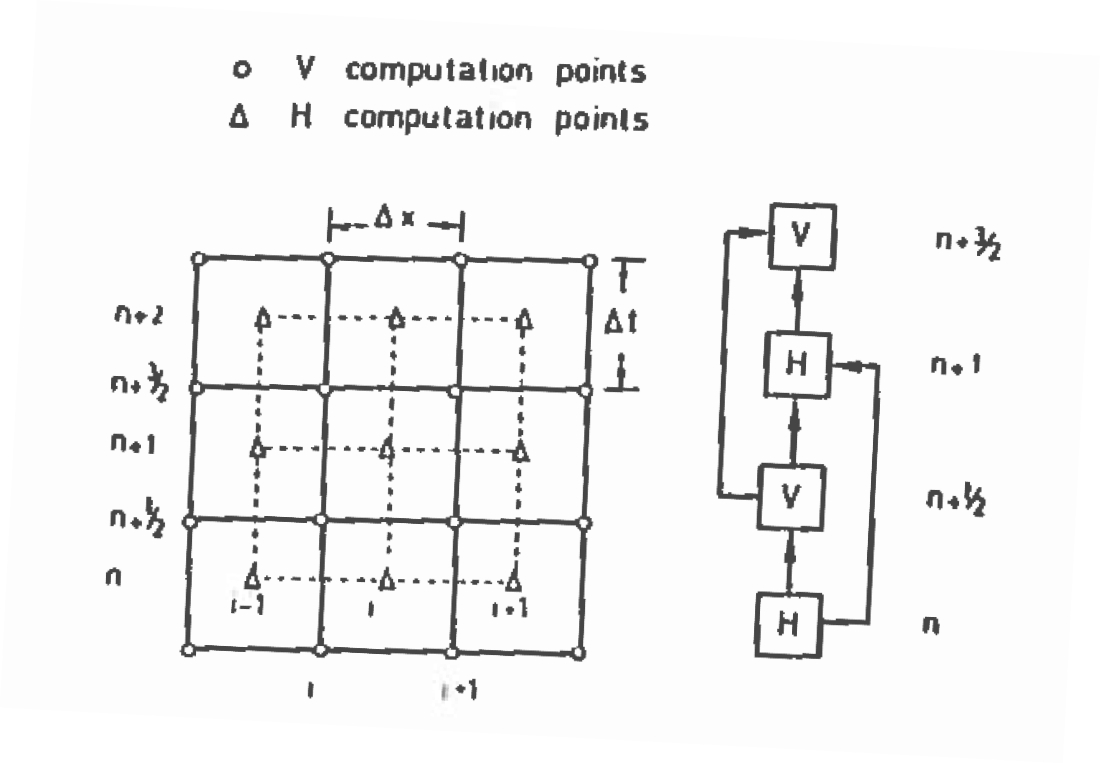
\includegraphics[width=6in]{./11-PipelineTransients/StaggeredSpaceTimeGrid.jpg} 
   \caption{Staggered grid (in space and time)}
   \label{fig:StaggeredSpaceTimeGrid}
\end{figure}

The figure depicts the spatial dimension along the horizontal axis.  
Each index value (i, i+1, i+2, \dots) labeled as a circle in the figure represents the interface between two ``rings, and fluid flow values are computed at these locations.  
Each index value labeled as a triangle in the figure represents the space within a ``ring'' and the head values are computed at these locations.   
Thus in the figure, location i (solid vertical lines) is the interface between rings i-1 and i. 
The values of head in the i-1 and i ring determine the velocity that traverses the ring interface.
For instance if the head in i-1 is larger than in ring i, flow should be from left to right in that time interval.

A similar staggered structure is depicted in the vertical time domain. 
Time levels are treated in the same fashion where all the head values are used to update velocity values, then these updated velocity values are in turn used to update the head values.

The boundary conditions are applied at each end of the computational domain -- Typically node 1 where head is a fixed value, and velocity depends on the head in node 2, and node N, where velocity is determined from the valve model, and head at N-1 is computed.

The application of the finite-difference equations to the linearized set of partial differential equations for any interior node (of either type) is
\begin{gather}
\begin{matrix}
\frac{V_i^{n+3/2}-V_i^{n+1/2}}{\Delta t}  &+~g\frac{H_i^{n+1}-H_{i-1}^{n+1/2}}{\Delta x} &+~\frac{fV_i^{n+1/2}|V_i^{n+1/2}|}{2d} &= & 0 \\
\\
\frac{H_i^{n+1}-H_i^{n}}{\Delta t}  &+~\frac{c^2}{g}\frac{V_{i+1}^{n+1/2}-V_{i}^{n+1/2}}{\Delta x} & &= & 0\\
\end{matrix}
\end{gather}
\newpage
\subsection{An Example \textbf{R} Implementation}
Figure \ref{fig:PipelineExample} is a sketch showing a pipeline supplied by a reservoir on the left with constant head of 5 meters.  The reservoir will be quite large relative to the volume in the pipeline -- think of Lake Mead on Boulder Canyon (Hoover Dam), and the pipeline is a supply pipe to a water treatment plant for a nearby community.

\begin{figure}[h!] %  figure placement: here, top, bottom, or page
   \centering
   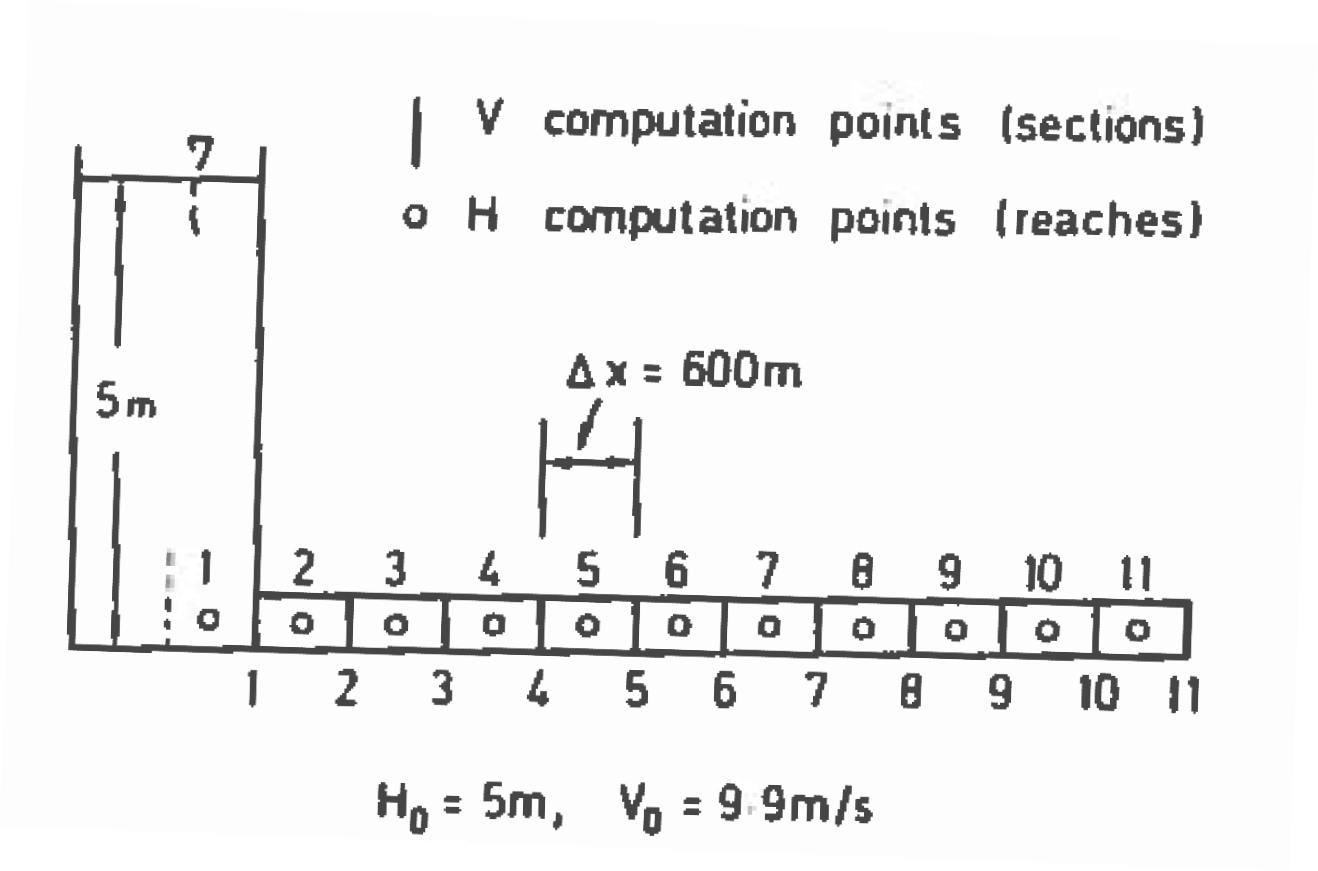
\includegraphics[width=6in]{./11-PipelineTransients/PipelineExample.jpg} 
   \caption{Pipeline with a constant head reservoir at the left side, and a valve shutdown at the right side}
   \label{fig:PipelineExample}
\end{figure}

The pipeline itself is 6 kilometers long (about 3.5 miles), with a diameter of 0.5 meters (about 18 inches) , and the pipe wall thickness is 4 millimeters (a little under 1/4 inch thick).  The steady flow velocity with the valve open is 9.9 meters/second (30 feet per second -- really fast for real pipes).

The valve is closed over a 2 second interval, with linear decrease in outlet area during the closure.  Neglecting frictional losses in the system, compute and plot the pressures at the valve for a 250-second duration. 

The script to accomplish these computations is shown in Listing \ref{lst:PipeTransientCode}. 
The code includes provision for the friction term, here we will just set it to zero.  
The code also sets time step size based on the Courant condition.  
The Courant number must equal unity for the algorithm to be stable.  
\newpage
\begin{lstlisting}[caption=R Code to compute for a pipeline transient example \\ , label=lst:PipeTransientCode]
##########################################################################################
# Pipeline Transients using Explicit Finite Differences (linearized formulation)         #
##########################################################################################
rm(list=ls()) # deallocate memory
######## prototype functions ###############
celerity <- function(density,elasticity_fluid,elasticity_solid,diameter,thickness){
  temp1<- 1.0/elasticity_fluid
  temp2<- diameter/(elasticity_solid*thickness)
  temp3<- temp1 + temp2
  temp4<- density*temp3
  celerity <- sqrt(1.0/temp4)
  return(celerity)
}
### Simulator Code ##############################
# Simulation Conditions (this section could be replaced with an input file)
# fluid properties
density <- 1000  #kg/m^3
elasticity_fluid <-   2.0e09 #Pa
elasticity_solid <- 160.0e09 #Pa
diameter <-  0.500 #m
thickness <- 0.004 #m
cc <- celerity(density,elasticity_fluid,elasticity_solid,diameter,thickness)
print(cc)
# simulation properties
deltax <- 600 #meters
courantRatio <- 0.99 #select courant ratio to set time step.  If bigger than 1 unstable
deltat <- courantRatio*(deltax/cc) # force to be courant number for stability
# allocate head and velocity vectors, assign initial values
startHead <- 5.0 #meters
startVelo <- 9.9 #meters/second
pipeLength <- 6000 #meters
closeTime <- 2.0 #seconds
simulationDuration <- 250 #seconds
frictionFactor <- 0.015 #Moody Chart
cellCount <- as.integer((pipeLength/600)+1)
head <- numeric(0)
velocity <- numeric(0)
for(i in 1:cellCount){
      head[i]<-startHead
  velocity[i]<-startVelo
}
# useful constants
dtdx <- deltat/deltax
cc2g <- cc^2/9.81
do2 <- 1.0/(diameter*2) #used when friction included
# allocate some output vectors
etime<-numeric(0)
headvalve<-numeric(0)
velocitytank<-numeric(0)
# simulation values
etime[1] <- 0
headvalve[1] <- head[cellCount]
velocitytank[1] <-velocity[1]
######################
# Time Stepping Loop #
######################
maxiter <- 1+simulationDuration/deltat
for(itime in 2:maxiter){
  etime[itime]<-etime[itime-1]+deltat
###### valve closure model ##############
  closeRatio <- 1.0 - (etime[itime]/closeTime)
  if(closeRatio >= 0.0){
  velocity[cellCount] <- closeRatio*sqrt(2*9.8*(head[1]))
  }
  else{
  velocity[cellCount] <- 0
  }
####### update velocity #########
for(i in 1:(cellCount-1)){
  friction <- frictionFactor*velocity[i]*abs(velocity[i])*do2
  velocity[i]=velocity[i]-9.81*dtdx*(head[i+1]-head[i])-deltat*friction
}
####### update head #########
for(i in 2:(cellCount)){
  head[i]=head[i]-cc2g*dtdx*(velocity[i]-velocity[i-1])
}
headvalve[itime]<-head[cellCount]
velocitytank[itime] <-velocity[1]
}
# report results
message("Maximum head at valve : ",max(headvalve))
message("Minimum head at valve : ",min(headvalve))
# plot results
par(mfrow=c(2,1))
plot(etime,headvalve,type="l",pch=19,lwd=3,tck=1,xlab="Time (seconds)",ylab="Head at Valve (meters)",col="red")
plot(etime,velocitytank,type="l",pch=19,lwd=3,tck=1,xlab="Time (seconds)",ylab="Velocity at Tank (meters/sec)",col="blue")
\end{lstlisting} 

The listing seems elaborate, but it is relatively simple.
First is a prototype function for the celerity. 
Next material properties and simulation characteristics are supplied.  
For the code to be more general, one would probably move a lot of these assignments into a file read structure.

Once everything is ready, the algorithm begins time-stepping. 
Within any single time step the following activities are performed:
\begin{enumerate}
\item Determine the downstream velocity at the valve based on the required closure model.
\item Update the velocity in each interior interface (1 to the section before the valve).
\item Update the head in each interior cell (2 to the last cell, which is upstream of the valve).
\item Record the head at the valve, and the velocity at the tank exit.
\end{enumerate}
 When the requisite time steps are completed, then report and plot the results.
 
Figure \ref{fig:PipelineExampleResult} is the example presented herein using \textbf{R Studio}.
The friction factor was set to 0, and the courant ratio was set to 1.
The head at the valve oscillates from $+\Delta~H$ to $-\Delta~H$, and the velocity repeatedly changes direction an value from +9.9 t0 -9.9 meters per second, exactly phase shifted relative to head by one-half cycle.
The time for the values to change is twice the pipeline length divided by the wave speed.

\begin{figure}[h!] %  figure placement: here, top, bottom, or page
   \centering
   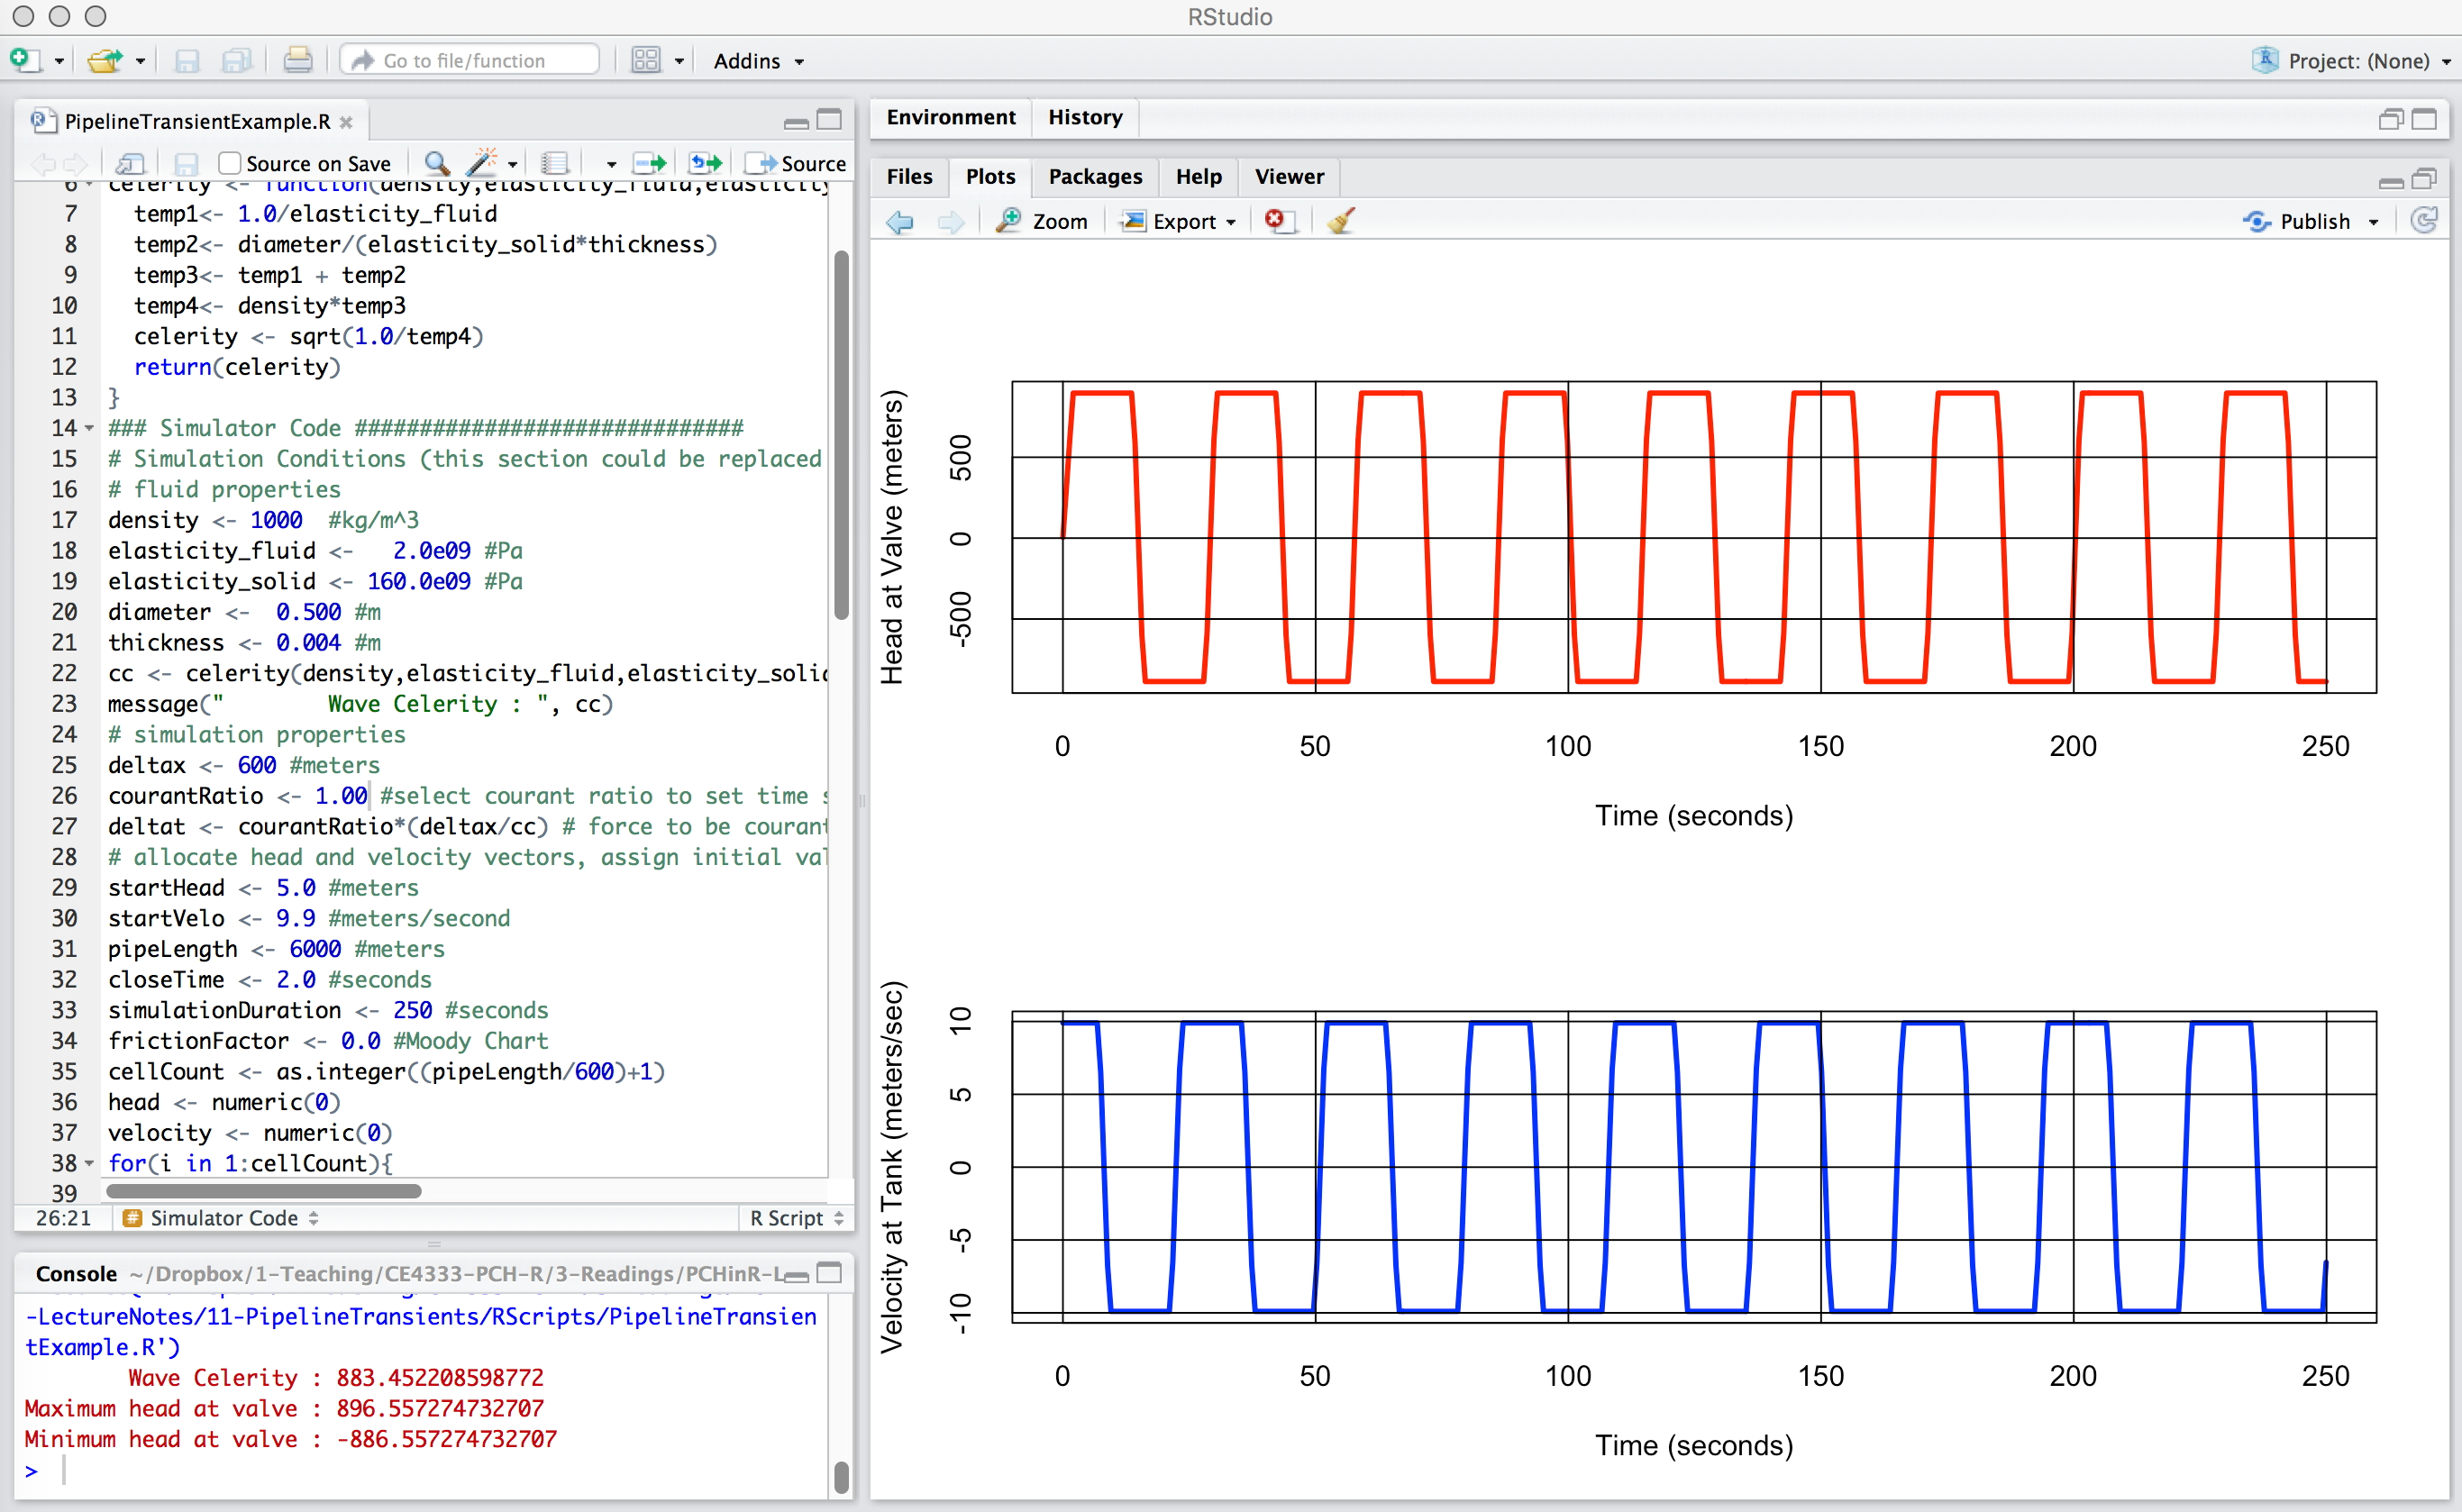
\includegraphics[width=6in]{./11-PipelineTransients/ExampleResult.jpg} 
   \caption{Pipeline transient simulation}
   \label{fig:PipelineExampleResult}
\end{figure}

Now if we add the friction term say $f=0.015$ which would be a value for a smooth pipe (especially at the flow velocities in the example) the effect of frictional damping is evident in the simulation and is displayed in 
Figure \ref{fig:PipelineExampleFriction}

\begin{figure}[h!] %  figure placement: here, top, bottom, or page
   \centering
   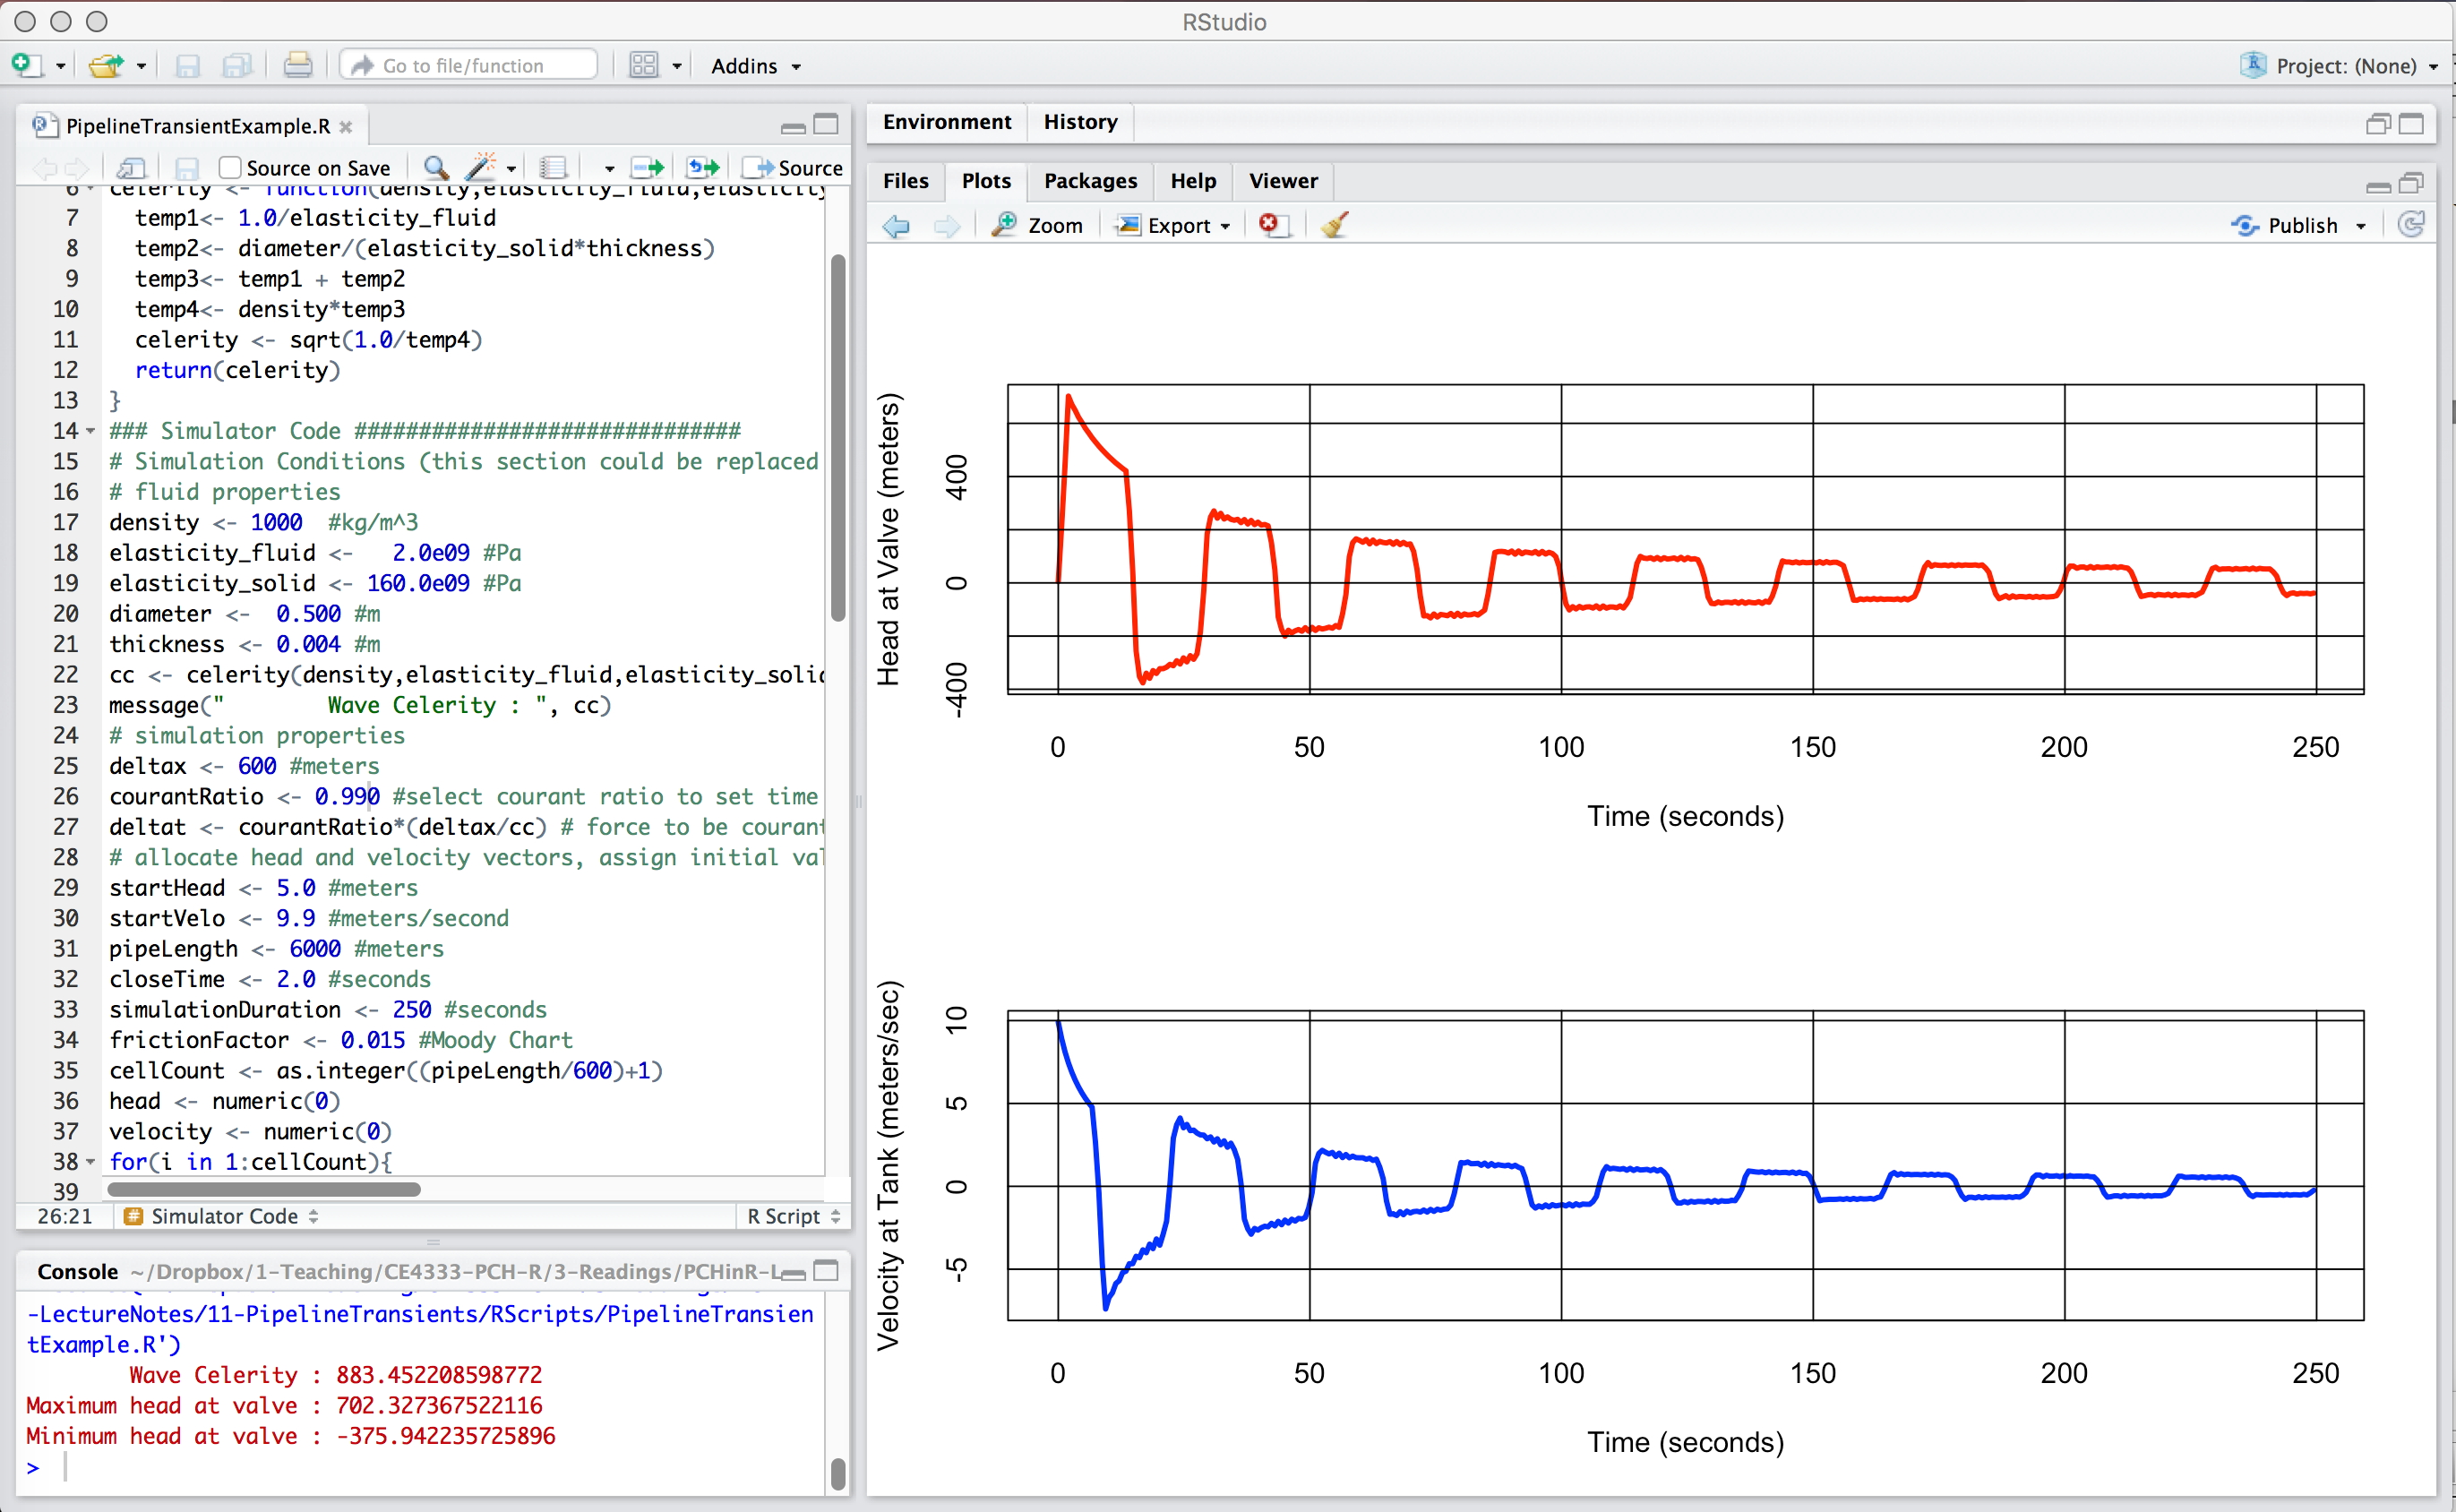
\includegraphics[width=6in]{./11-PipelineTransients/ExampleResultFriction.jpg} 
   \caption{Pipeline simulation with friction}
   \label{fig:PipelineExampleFriction}
\end{figure}

%\section*{Exercises}
%\begin{enumerate}
%\item Repeat the example problem presented in class and the textbook except modify the code for a frictionless, instantaneous valve closure. 
%\item Repeat the example problem for a friction factor of 0.016, and instantaneous valve closure.
%\item Repeat the example problem with a friction factor of 0.016, and a 1-second valve closure.  Change the ``ring'' length to 60 meters (instead of 600 in the example).  Use the largest Courant ratio that produces a stable result, for a 300 second long simulation.  What does the output trace look like as compared to the 60 meter long computation element?
%\item Repeat the above problem, except assume the pipe wall thickness is 25 millimeters.  What effect does this change in material property have on the simulation result?
%\item Suppose the steel pipe is replaced with a thin wall polymer pipe (thickness 4 millimeters), with elastic modulus ten times greater than water, what effect do these material property changes have on the simulation result?
%\end{enumerate}

\subsection*{Exercises}
Exercise Set ES-9 On Class Server
